\documentclass[9pt, compress, aspectratio=169]{beamer}

\usepackage[sfdefault]{plex-sans}
\usepackage{xcolor}
\usepackage{array}
\usepackage{booktabs}
\usepackage{qrcode}
\usepackage{tikz}

\definecolor{links}{HTML}{F54927}
\hypersetup{colorlinks,linkcolor=,urlcolor=links,citecolor=gray}

% Citations as gray superscripts: text^[1]
\let\oldcite\cite
\renewcommand{\cite}[1]{\textsuperscript{\oldcite{#1}}}

% Allow for denser spacing globally
\setbeamertemplate{itemize/enumerate body begin}{\setlength{\leftmargini}{1.5em}\setlength{\itemsep}{2pt}}
\setbeamertemplate{navigation symbols}{}

% Numbered references: [1], [2], ... instead of beamer's book icons
\setbeamertemplate{bibliography item}{\insertbiblabel}
\setbeamertemplate{frametitle continuation}{}
\setbeamerfont{bibliography item}{size=\scriptsize}
\setbeamerfont{bibliography entry author}{size=\scriptsize}
\setbeamerfont{bibliography entry title}{size=\scriptsize}
\setbeamerfont{bibliography entry location}{size=\scriptsize}
\setbeamerfont{bibliography entry note}{size=\scriptsize}

% Add footer with title and slide number
\setbeamertemplate{footline}{
  \leavevmode%
  \hbox{%
    \begin{beamercolorbox}[wd=.7\paperwidth,ht=3ex,dp=2ex,left,leftskip=4ex]{author in head/foot}%
      \footnotesize HackerFab IITB: EE669 Guest Lecture
    \end{beamercolorbox}%
    \begin{beamercolorbox}[wd=.3\paperwidth,ht=3ex,dp=2ex,right,rightskip=4ex]{page number in head/foot}%
      \footnotesize \insertframenumber{} / \inserttotalframenumber
  \end{beamercolorbox}}%
  \vskip1ex%
}

% Custom commands for side-by-side content
\newcommand{\splitslide}[3][0.7]{
  \begin{columns}[T]
    \begin{column}{#1\textwidth}
      #2
    \end{column}
    \begin{column}{\dimexpr\textwidth-#1\textwidth\relax}
      \centering
      #3
    \end{column}
  \end{columns}
}

\newcommand{\slidepic}[2]{
  \includegraphics[width=0.95\linewidth,keepaspectratio]{#1}\\
  \vspace{0.06em}
  {\scriptsize \textit{#2}}\\
}

% Two photos side by side at a common height: {height}{img1}{caption1}{img2}{caption2}
\newcommand{\picpair}[5]{
  \begin{tabular}{@{}c@{\hspace{0.3cm}}c@{}}
    \includegraphics[height=#1]{#2} & \includegraphics[height=#1]{#4} \\
    {\scriptsize \textit{#3}} & {\scriptsize \textit{#5}}
  \end{tabular}
}

% Image for table cells
% Image tile for the slide-3 grid: {number}{file}{label}
\newcommand{\gridpic}[3]{\parbox[t]{2.6cm}{\centering\includegraphics[width=2.6cm,height=1.85cm,keepaspectratio]{#2}\\[1pt]{\tiny #1. #3}}}

% Wrapper for slides
\newenvironment{slide}[1]{
  \begin{frame}[environment=slide, t]
    \frametitle{#1}
  }{
  \end{frame}
}

\newcommand{\setupimg}{media_my/04_lab_photos/litho setup latest.jpg}
\newcommand{\resimg}{media_my/04_lab_photos/litho 3um resolution.jpg}

\begin{document}

%% ---------------------------------------------------------------- Title
\begin{frame}[t]
  \vspace{-0.3cm}
  \begin{columns}[T]
    \begin{column}{0.78\textwidth}
      \begin{flushleft}
        {\footnotesize HackerFab Guest Lecture \textbar{} 05-11-2026 \textbar{} Jai Bellare}\\[2pt]
        {\footnotesize For EE669 \textbar{} Prof.\ Anil Kottantharayil}\\[0.4cm]
        {\Large \textbf{Design and Development of a \textless\$2000\\[2pt] Direct-Write Photolithography System}}
      \end{flushleft}
    \end{column}
    \begin{column}{0.22\textwidth}
      \begin{flushright}
        \qrcode[nolink,height=1.7cm]{https://hackerfabiitb.org/}\\[2pt]
        {\scriptsize \href{https://hackerfabiitb.org/}{hackerfabiitb.org}}
      \end{flushright}
    \end{column}
  \end{columns}

  \vfill
  \centering
  \picpair{4.3cm}{\setupimg}{Direct-write photolithography setup}{\resimg}{3 µm lines patterned by our system}
  \vspace{0.1cm}
\end{frame}

%% ---------------------------------------------------------------- About (slide 1 of funding_proposal/presentation.tex)
\begin{frame}[t]
  \vspace{-0.5cm} % Reduce margin above the title
  \begin{columns}[T]
    \begin{column}{0.65\textwidth}
      \begin{flushleft}
        {\Large \textbf{HackerFab IITB}} \\
        {\normalsize \vspace{2pt} \textit{democratizing semiconductor fabrication}} \\
      \end{flushleft}
    \end{column}
    \begin{column}{0.35\textwidth}
      \begin{flushright}
        \vspace{-0.3cm}
        \includegraphics[width=0.6\linewidth]{media_claude/template/logo.png}\\[0.2em]
        {\scriptsize \href{https://hackerfabiitb.github.io/}{hackerfabiitb.github.io}\\
          \vspace{-0.1cm}
        \href{mailto:hackerfabiitb@gmail.com}{hackerfabiitb@gmail.com}}
      \end{flushright}
    \end{column}
  \end{columns}

  \vspace{0.1cm}
  \hrule
  \vspace{0.15cm}

  {\small
    \begin{enumerate}
        \setlength\itemsep{2pt}
      \item \textbf{Who we are:}  A student-led R\&D project guided by IIT Bombay SemiX faculty.
        We are building low-cost open-source student-accessible tools for making chips and transistors.
      \item \textbf{Our Mission:} To develop a low-cost DIY semiconductor fab capable of making working transistors, whose open-source recipe can be replicated and developed by colleges across India.
      \item \textbf{Our Vision:} To empower every EE student in India to learn to fabricate semiconductor devices (like a Tinkerer's Lab or Makerspace for semiconductors)
      \item \textbf{Advised by SemiX faculty:} Prof. Swaroop Ganguly, Prof. Udayan Ganguly, Prof. Anil Kottantharayil and Prof. Veeresh Deshpande
      \item \textbf{Recognition:}\par
        \begin{minipage}[t]{0.63\linewidth}
          \begin{enumerate}
            \item won User Design Track at 39th International Conf. On VLSI Design for our DIY toolkit \& \textbf{Fab-in-a-Box} proposal
            \item \href{https://swarajyamag.com/technology/inside-hackerfab-iitb-indias-first-student-led-chip-fab}{Interview and article by Swarajya Magazine}\cite{swarajya}
            \item \href{https://x.com/RuntimeBRT/status/2070061936407195654}{Deep-dive video by RuntimeBRT}\cite{runtime}
          \end{enumerate}
        \end{minipage}\hfill
        % headline strip cropped out of the full Swarajya article screenshot
        \begin{minipage}[t]{0.3\linewidth}
          \vspace{0pt}
          \includegraphics[width=\linewidth,trim=0 811bp 0 0,clip]{media_claude/template/2026-08-17_01-57-42 swarajya.png}
        \end{minipage}
  \end{enumerate}}
\end{frame}

%% ---------------------------------------------------------------- Range of litho systems
\begin{slide}{Range of Lithography Systems}
  \vspace{0.25cm}
  \begin{columns}[c]
    \begin{column}{0.62\textwidth}
      {\footnotesize
        \setlength{\tabcolsep}{3.5pt}
        \renewcommand{\arraystretch}{1.45}
        \begin{tabular}{>{\centering\arraybackslash}m{0.35cm} >{\raggedright\arraybackslash}m{2.65cm} >{\centering\arraybackslash}m{1.15cm} >{\centering\arraybackslash}m{1.45cm} >{\centering\arraybackslash}m{1.6cm}}
          \toprule
          \textbf{Sr No} & \textbf{Tool Name} & \textbf{Resolution (nm)} & \textbf{Throughput (wafers/hr)} & \textbf{Cost (USD)} \\
          \midrule
          1 & ASML TWINSCAN EXE:5200B \newline {\scriptsize High-NA EUV scanner}\cite{asml,toms}
            & 8 & 175 & \$380M \\
          2 & IMS MBMW-101 / -301 \newline {\scriptsize multi-beam mask writer}\cite{ims,semieng,dataintelo}
            & 14 & 0.1 \newline {\scriptsize \emph{masks}/hr} & \$80M \\
          3 & Raith VOYAGER \newline {\scriptsize 50 kV e-beam lithography}\cite{raith}
            & 8 & 0.02 & \$5M \\
          4 & Durham Magneto Optics MicroWriter ML3 Pro \newline {\scriptsize maskless laser direct-write}\cite{dmo,nus}
            & 600 & 0.4 & \$0.5M \\
          5 & \textbf{HackerFab IITB Litho} \newline {\scriptsize DMD projection direct-write}
            & 3000 & 0.003 & \textbf{\$2k} \\
          \bottomrule
        \end{tabular}
      }
    \end{column}
    \begin{column}{0.38\textwidth}
      \centering
      \gridpic{1}{media_claude/asml_exe5200b.png}{ASML EXE:5200B}\hfill
      \gridpic{2}{media_claude/ims_mbmw101.jpg}{IMS MBMW-101}\\[0.2cm]
      \gridpic{3}{media_claude/raith_voyager_crop.jpg}{Raith VOYAGER}\hfill
      \gridpic{4}{media_my/microwriter.png}{MicroWriter ML3}\\[0.2cm]
      \gridpic{5}{\setupimg}{HackerFab Litho}
    \end{column}
  \end{columns}
\end{slide}

%% ---------------------------------------------------------------- ASML EUV
\begin{slide}{ASML EUV}
  \centering
  \includegraphics[width=0.8\linewidth,height=0.72\textheight,keepaspectratio]{media_claude/asml_euv_cnbc.jpg}\\
  {\scriptsize \textit{ASML NXE:3400B EUV scanner (CNBC)}\cite{cnbc}}
\end{slide}

%% ---------------------------------------------------------------- HackerFab Litho
\begin{slide}{HackerFab Litho}
  \vspace{0.4cm}
  \centering
  \picpair{4.4cm}{\setupimg}{Direct-write photolithography setup}{\resimg}{3 µm lines patterned by our system}
\end{slide}

%% ---------------------------------------------------------------- Optical diagram
\begin{slide}{Optical Diagram}
  \centering
  \vspace{0.2cm}
  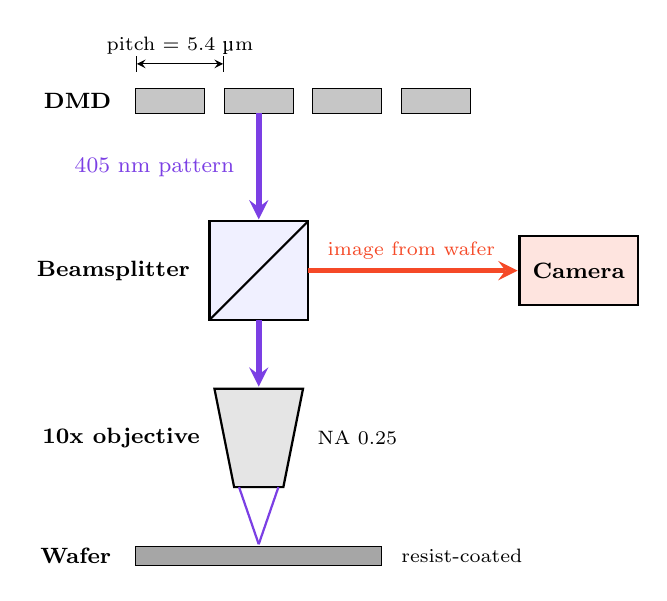
\begin{tikzpicture}[scale=1.25, >=stealth, every node/.style={font=\footnotesize}]
    \definecolor{uv}{HTML}{7B3FE4}
    \definecolor{cam}{HTML}{F54927}
    % DMD: 4 mirrors
    \foreach \i in {0,1,2,3}
      \fill[gray!45, draw=black] (\i*0.9, 6.2) rectangle ++(0.7, 0.25);
    \node[anchor=east] at (-0.15, 6.32) {\textbf{DMD}};
    \draw[|<->|, thin] (0, 6.7) -- (0.9, 6.7) node[midway, above] {\scriptsize pitch = 5.4 µm};
    % DMD -> beamsplitter
    \draw[uv, line width=2pt, ->] (1.25, 6.2) -- (1.25, 5.12);
    \node[anchor=east, text=uv] at (1.1, 5.65) {405 nm pattern};
    % beamsplitter
    \draw[thick, fill=blue!6] (0.75, 4.1) rectangle (1.75, 5.1);
    \draw[thick] (0.75, 4.1) -- (1.75, 5.1);
    \node[anchor=east] at (0.65, 4.6) {\textbf{Beamsplitter}};
    % beamsplitter -> objective
    \draw[uv, line width=2pt, ->] (1.25, 4.1) -- (1.25, 3.42);
    % objective
    \draw[thick, fill=gray!20] (0.8, 3.4) -- (1.7, 3.4) -- (1.5, 2.4) -- (1.0, 2.4) -- cycle;
    \node[anchor=east] at (0.75, 2.9) {\textbf{10x objective}};
    \node[anchor=west] at (1.75, 2.9) {\scriptsize NA 0.25};
    % focus onto wafer
    \draw[uv, thick] (1.05, 2.4) -- (1.25, 1.82);
    \draw[uv, thick] (1.45, 2.4) -- (1.25, 1.82);
    % wafer
    \fill[gray!70, draw=black] (0, 1.6) rectangle (2.5, 1.8);
    \node[anchor=east] at (-0.15, 1.7) {\textbf{Wafer}};
    \node[anchor=west] at (2.6, 1.7) {\scriptsize resist-coated};
    % beamsplitter -> camera
    \draw[cam, line width=2pt, ->] (1.75, 4.6) -- (3.88, 4.6);
    \node[above, text=cam] at (2.8, 4.62) {\scriptsize image from wafer};
    \draw[thick, fill=cam!15] (3.9, 4.25) rectangle (5.1, 4.95);
    \node at (4.5, 4.6) {\textbf{Camera}};
  \end{tikzpicture}
\end{slide}

%% ---------------------------------------------------------------- DMD
\begin{slide}{Digital Micromirror Device (DMD)}
  \centering
  \begin{tabular}{@{}c@{\hspace{0.6cm}}c@{}}
    \includegraphics[height=0.55\textheight,keepaspectratio]{media_my/ti_dlp.png} &
    \includegraphics[height=0.55\textheight,keepaspectratio]{media_claude/dmd_ieee_spectrum.jpg} \\
    {\scriptsize \textit{TI DLPDLCR471TPEVM evaluation module}} &
    {\scriptsize \textit{Close-up of DMD micromirrors (IEEE Spectrum)}\cite{ieeedmd}}
  \end{tabular}

  \vspace{0.3cm}
  {\small
    DLP471TP DMD\cite{ti471}: \textbf{5.4 µm mirror pitch}, 1920 $\times$ 1080 mirrors, $\pm$17° tilt, 0.47'' diagonal (10.37 $\times$ 5.83 mm)\\[2pt]
    With $\approx$10x demagnification: $\approx$0.54 µm pixel and $\approx$1.0 $\times$ 0.58 mm field on the wafer
  }
\end{slide}

%% ---------------------------------------------------------------- Optical specs
\begin{slide}{Optical Specs}
  \splitslide[0.42]{
    {\small
      \begin{enumerate}
          \setlength\itemsep{4pt}
        \item \textbf{Objective:} 10X DIN plan objective\cite{edmund}
          \begin{enumerate}
            \item NA = \textbf{0.25}
            \item EFL = 15.37 mm, WD = 1.5 mm
          \end{enumerate}
        \item \textbf{Wavelength:} $\lambda$ = \textbf{405 nm}
        \item \textbf{Diffraction limit:}
          \begin{enumerate}
            \item Airy disk diameter: $1.22\,\lambda/\mathrm{NA}$ = 1.98 µm
            \item Rayleigh resolution: $0.61\,\lambda/\mathrm{NA}$ = \textbf{0.99 µm}
          \end{enumerate}
        \item \textbf{Measured:} 3 µm lines, so $k_1 = \mathrm{CD}\cdot\mathrm{NA}/\lambda \approx 1.85$. The optics are not what limits us.
      \end{enumerate}
    }
  }{
    \raggedright
    {\small
      \textbf{Is $1.22\,\lambda/\mathrm{NA}$ the right formula?}
      \begin{enumerate}
          \setlength\itemsep{3pt}
        \item $1.22\,\lambda/\mathrm{NA}$ is the \emph{diameter} of the Airy disk, out to the first dark ring.
        \item Two points are just resolved when one sits on the other's first dark ring (Rayleigh criterion), so the resolution is the \emph{radius}: $0.61\,\lambda/\mathrm{NA}$.
        \item Lithography writes this as $\mathrm{CD} = k_1\,\lambda/\mathrm{NA}$.
      \end{enumerate}

      \smallskip
      \textbf{What sets the 1.22?}
      \begin{enumerate}
          \setlength\itemsep{3pt}
        \item \textbf{Pupil shape:} 1.22 = 3.83/$\pi$, the first zero of the Bessel function $J_1$, for a uniformly lit \emph{circular} aperture. A slit gives 1.0.
        \item \textbf{Criterion:} Rayleigh 0.61, Abbe 0.5, Sparrow 0.47.
        \item \textbf{Illumination coherence ($\sigma$):} coherent light resolves line/space down to a half-pitch of $0.5\,\lambda/\mathrm{NA}$; off-axis illumination gets down to $0.25\,\lambda/\mathrm{NA}$.
        \item \textbf{In practice:} aberrations, defocus, the resist and the process push $k_1$ higher.
      \end{enumerate}
    }
  }
\end{slide}

%% ---------------------------------------------------------------- How we built it
\begin{slide}{How we built Litho}
\end{slide}

%% ---------------------------------------------------------------- 10x objective question
\begin{slide}{Q] Why only a 10x objective? Why not use a 100x lens and get 500 nm resolution?}
\end{slide}

%% ---------------------------------------------------------------- Characterising performance
\begin{slide}{Characterising Performance of a Litho System}
  \begin{enumerate}
      \setlength\itemsep{6pt}
    \item Critical Dimension (CD) / Minimum Feature Size / Resolution
    \item Line/Space
    \item Latent Image
    \item Developed Image
  \end{enumerate}
\end{slide}

%% ---------------------------------------------------------------- Thanks
\begin{frame}[c]
  \centering
  {\Huge \textbf{Thank you!}}\\[0.6cm]
  {\Large Questions?}\\[0.8cm]
  \qrcode[nolink,height=1.8cm]{https://hackerfabiitb.org/}\\[2pt]
  {\scriptsize \href{https://hackerfabiitb.org/}{hackerfabiitb.org}}
\end{frame}

%% ---------------------------------------------------------------- References
\begin{frame}[t, allowframebreaks]
  \frametitle{References}
  \begin{thebibliography}{99}
    \bibitem{swarajya} Swarajya, ``Inside HackerFab IITB: India's first student-led chip fab.'' \url{https://swarajyamag.com/technology/inside-hackerfab-iitb-indias-first-student-led-chip-fab}
    \bibitem{runtime} RuntimeBRT, deep-dive video on HackerFab IITB. \url{https://x.com/RuntimeBRT/status/2070061936407195654}
    \bibitem{asml} ASML, ``TWINSCAN EXE:5200B'' product page. \url{https://www.asml.com/en/products/euv-lithography-systems/twinscan-exe-5200b}
    \bibitem{toms} Tom's Hardware, ``ASML's roadmap for chipmaking lithography tools examined.'' \url{https://tomshardware.com/tech-industry/semiconductors/asml-lithograpy-roadmap-examined-from-duv-to-hyper-na}
    \bibitem{ims} IMS Nanofabrication, ``Products: Multi-Beam Mask Writer.'' \url{https://www.ims.co.at/en/products/}
    \bibitem{semieng} Semiconductor Engineering, ``Multi-Beam Mask Writing Finally Comes Of Age.'' \url{https://semiengineering.com/multi-beam-mask-writing-finally-comes-of-age}
    \bibitem{dataintelo} Dataintelo, ``Multibeam Mask Writers Market Research Report.'' \url{https://dataintelo.com/report/global-multi-beam-mask-writer-market}
    \bibitem{raith} Raith, ``VOYAGER: e-beam lithography system.'' \url{https://raith.com/products/voyager/}
    \bibitem{dmo} Durham Magneto Optics, ``MicroWriter ML3 Pro.'' \url{https://www.durhammagnetooptics.com/?product=microwriter}
    \bibitem{nus} NUS E6 Nanofab, ``MicroWriter: Durham Magneto Optics ML3 Pro.'' \url{https://cde.nus.edu.sg/e6nanofab/microwriter-durham-magneto-optics-ml3-pro-class-10}
    \bibitem{cnbc} CNBC, image of ASML NXE:3400B EUV scanner. \url{https://encrypted-tbn0.gstatic.com/images?q=tbn:ANd9GcTTk3zVFs2LxehMMxF3rxeBNKeXYQnqXPUWnc33hxwZ4Q&s=10}
    \bibitem{ieeedmd} IEEE Spectrum, close-up of a digital micromirror device. \url{https://spectrum.ieee.org/media-library/close-up-of-microscopic-square-tiles-with-holes-in-the-center-arranged-in-a-grid-pattern.jpg?id=25583281}
    \bibitem{ti471} Texas Instruments, ``DLP471TP 0.47 4K UHD DMD'' datasheet (DLPS173B). \url{https://www.ti.com/lit/gpn/DLP471TP}
    \bibitem{edmund} Edmund Optics, ``10X DIN Plan Commercial Grade Objective.'' \url{https://www.edmundoptics.in/p/10x-din-plan-commercial-grade-objective/5386}
  \end{thebibliography}
\end{frame}

\end{document}
